% !TeX program = xelatex
% !Mode:: "TeX:UTF-8"
%%  本模板推荐以下方式编译: xelatex
%%     1. 文件默认的编码为 UTF-8 对于windows,请选用支持UTF-8编码的编辑器。
%%   2. 若是模板有什么问题,请及时与我们取得联系,Email:latexstudio@qq.com。
%%   3. 可以到  https://ask.latexstudio.net 提问
%%   4. 请安装 最新版本的 TeXLive 地址:
%%   http://mirrors.ctan.org/systems/texlive/Images/texlive.iso

\documentclass[12pt,a4paper]{nmmcm}
\usepackage{ctex}
\usepackage{graphicx}
\usepackage{booktabs,colortbl}
\usepackage{xcolor}
\usepackage{tikz}
\usepackage{indentfirst}
\mcmsetup{CTeX = true,
        tcn ={\xiaowuhao 2023000000001 }(\textcolor{red}{\textit{需要修改为自己队伍的实际队号}}), problem = A,
        sheet = true, titleinsheet = false, keywordsinsheet = true,
        titlepage = true, abstract = true}
\usepackage{xurl}
\setmainfont{Times New Roman}
\setmonofont[
    Path=fonts/,
    UprightFont = *-Regular,
    BoldFont = *-Bold,
    ItalicFont = *-Italic
]{UbuntuMono}
\usepackage{lipsum}


\usepackage{paralist}
\let\itemize\compactitem
\let\enditemize\endcompactitem
\let\enumerate\compactenum
\let\endenumerate\endcompactenum
\let\description\compactdesc
\let\enddescription\endcompactdesc

\setlength\abovedisplayskip{5pt}
\setlength\belowdisplayskip{-8pt}
\setlength{\parskip}{0.1em}

\newcommand\wordc[1]{\textbf{#1}}
\renewcommand{\appendixtocname}{附\quad录}
\renewcommand{\appendices}{\hspace{-2em}{\sanhao\HEI {\bf 附~~~录}}}
\colorlet{tableheadcolor}{gray!25} % Table header colour = 25% gray
\newcommand{\headcol}{\rowcolor{tableheadcolor}}

\title{\textcolor{red}{论文的题目(三号黑体)}}
\date{}

\usepackage[font=small,labelfont={bf,sf},tableposition=top]{caption}


\begin{document}
\begin{abstract}


%abstract---------------
{\song\xiaosihao
\setlength{\parindent}{2em}\textcolor{red}{(第1段)	问题重述+简要思想:首先简要叙述所给问题的背景和动机,并分别分析每个小问题的特点(以下以三个问题为例)。根据这些特点说出自己的思想:针对于问题1,采用~$\cdots \cdots$ 的方法解决;针对问题2用~$\cdots \cdots$ 的方法解决;针对问题3用~$\cdots \cdots$ 的方法解决。}


\setlength{\parindent}{2em}\textcolor{red}{(第2段)	模型建立及求解结果:介绍思想和模型: 对于问题1我们首先建立了~$\cdots \cdots$ 模型I。首先利用~$\cdots \cdots$ ,其次计算了~$\cdots \cdots$ ,并借助~$\cdots \cdots$ 数学算法和~$\cdots \cdots$ 软件得出了~$\cdots \cdots$ 结论。}

\setlength{\parindent}{2em} \textcolor{red}{(第3段)	对于问题2我们用~$\cdots \cdots$(模型的建立与求解结果的陈述中,思想、模型、软件和结果必须描述清晰,亮点详细说明需突出。}

\setlength{\parindent}{2em}\textcolor{red}{(第4段)	对于问题3我们用~$\cdots \cdots$ (模型的建立与求解结果的陈述中,思想、模型、软件和结果必须描述清晰,亮点详细说明需突出。}

\setlength{\parindent}{2em}\textcolor{red}{(第5段)	优化结果及总结:在~$\cdots \cdots$ 条件下,针对~$\cdots \cdots$ 模型进行适当修改与优化,这种条件的改变可能来自你的一种猜想或建议。要注意合理性。此推广模型可以不深入研究,也可以没有具体结果。}
}

\begin{rmk}
    字数300$\sim $600之间,需控制在一页;摘要中必须将具体方法、模型和所得结果写出来;摘要要求“总分总”,段开头可用“针对问题1,针对问题2,针对问题3..”或者“首先,然后,其次,最后”等词语进行有逻辑的论述。摘要是重中之重,必须严格执行!
\end{rmk}







\begin{keywords}
{\song\xiaosihao
\textcolor{red}{使用到的模型名称、方法名称、特别是亮点一定要在关键字里出现,3$\sim$ 5个较合适。}}
\end{keywords}

\begin{itemize}
  \item \textcolor{blue}{前面一页必须使用模板格式(黑色部分),否则论文检测不通过。}
  \item \textcolor{blue}{ 目录页为论文开始处,论文正文用阿拉伯数字从“1”开始连续编号,页码位于每页页脚中部。(鼓励使用目录)}
\end{itemize}

\end{abstract}
\maketitle
\renewcommand{\contentsname}{\centerline{\sanhao\bfseries\HEI 目\quad 录}}
%\thispagestyle{empty}
%{\song\xiaosihao
\tableofcontents
%}

\newpage
\setcounter{page}{1}
\pagestyle{fancy}
\section{问题重述}
\subsection{引言}
%Introduction---------------

\setlength{\parindent}{2em} 
在本研究中,依据地质资源勘探部门在特定海域内的14个钻孔勘探数据,这些数据包括每个钻孔的具体位置、深度以及相应深度的孔隙度和天然气水合物饱和度的测量信息。本研究旨在:

1)确定研究区域内天然气水合物的资源分布范围;

2)评估区域内资源参数如有效厚度、地层孔隙度和饱和度的概率分布及其变化规律;

3)基于统计分析提出天然气水合物资源量的概率分布估计;

4)针对资源评估的进一步精细化,提出在研究区域增加钻探井位的策略。

\subsection{要解决的具体问题}
\begin{enumerate}
  \item \textcolor{red}{问题一:问题一的重述,重述语言简洁明了,突出模型中第一个要解决的问题,突出核心。}
  \item \textcolor{red}{问题二:问题二的重述。}
  \item \textcolor{red}{问题三:问题三的重述。}
  \item \textcolor{red}{问题四:问题四的重述。}
\end{enumerate}

\section{问题分析}

\textcolor{red}{主要是表达对题目的理解,特别是对附件的数据进行必要分析、描述(一般都有数据附件),这是需要提到分析数据的方法、理由。如果有多个小问题,可以对每个小问题进行分别分析。问题分析中不给出结果,结果在摘要中给出。
(假设有2个问题)}

\subsection{问题一的分析}

 \textcolor{red}{对问题1研究的意义的分析。
问题1属于$\cdots\cdots$数学问题,对于解决此类问题一般数学方法的分析。
对附件中所给数据特点的分析。
对问题1所要求的结果进行分析。
由于以上原因,我们可以将首先建立一个$\cdots\cdots$的数学模型I,然后将建立一个$\cdots\cdots$的模型II,$\cdots\cdots$对结果分别进行预测,并将结果进行比较.
}


\subsection{问题二的分析}
 \textcolor{red}{对问题2研究的意义的分析。
问题2属于$\cdots\cdots$数学问题,对于解决此类问题一般数学方法的分析。
对附件中所给数据特点的分析。
对问题2所要求的结果进行分析。
由于以上原因,我们可以将首先建立一个$\cdots\cdots$的数学模型I,然后将建立一个$\cdots\cdots$的模型II,$\cdots\cdots$对结果分别进行预测,并将结果进行比较.
}

 $\cdots\cdots$


\section{模型假设}
\begin{enumerate}
  \item 模型的假设要结合整个模型的建立作出的一个合理的假设,不能过于理想化,要尽量切合实际问题的处理来做出相应的合理的假设;
  \item 模型假设二;
  \item 模型假设三;
\end{enumerate}

\section{名词解释与符号说明}

\textcolor{red}{一般都会有符号解释和说明,对于一些装有的专有名词解释,需要的时候就需要对其进行解释与说明,我们以下面几个例子为例。}

\subsection{名词解释与说明}
\begin{enumerate}
\item \wordc{理论通行能力:}理论通行能力是指每一条车道~(或每一条道路) 在单位时间内
能够通过的最大交通量。

\begin{figure}[h!t]
\centerline{
\includegraphics[scale=0.4]{gonghao}}
\caption{  图~1的标题名称}
\end{figure}

关于插图、绘图、表格以及公式等相关资源请点击~\href{http://www.latexstudio.net}{\textcolor{blue}{\LaTeX{}工作室}}

\item \wordc{修正通行能力:}在具体条件下,通过修正系数对理论通行能力修正后得到的单
位时间内所能通过的最大交通量。

\end{enumerate}
\subsection{主要符号与说明}

%tab1
\begin{table}[h!]
  \centering
  \small
  \begin{tabular}{p{60pt}<{\centering}|p{60pt}<{\centering}p{180pt}<{\raggedright}}
   \hline
   \headcol 序号 & 符号 & 符号说明 \\
   \hline
    1 & $\nu$ & 行车速度(km/h) \\
    2 & t$_{\min}$ & 车头最小时距(s) \\
    3 & $J_{\rm a}$ & 车头最小间隔(m) \\
    4 & $J_{\rm z}$ & 车辆平均长度(m) \\
    5 & $J_{\gamma}$ & 车辆的制动距离(m) \\
    6 & $J_{\max}$ & 司机在反应时间内车辆行驶的距离(m) \\
    7 & $A_{\max}$ & 最大交通量 \\
    8 & $\alpha_{1}$ & 车道数修正系数 \\
    9 & $\alpha_{2}$ & 车道宽度和侧向净宽修正系数 \\
    10 & $\alpha_{3}$ & 大型车修正系数 \\
    11 & $\alpha_{4}$ & 驾驶员技术水平修正系数 \\
    12 & $K_{j}$ & 阻塞密度 \\
    13 & $\nu_{f}$ & 自由车速 \\
    $\cdots$ & $\cdots$\\
    \hline
  \end{tabular}
  %\caption{符号与说明}
  \label{symbol}
\end{table}

\section{模型的建立与求解}

数据的预处理:
1. $\cdots\cdots$数据全部缺失,不予考虑。
2. 对数据测试的特点,如周期等进行分析。
3. $\cdots\cdots$数据残缺,根据数据挖掘等理论根据$\cdots\cdots$变化趋势进行补充。
4. 对数据特点(后面将会用到的特征)进行提取。
   用$\cdots\cdots$软件聚类分析和各个不同问题的需要,采得$\cdots\cdots$组采样,每组5-8个采样值。将采样所对应的特征值进行列表或图示。
根据数据特点,对总体和个体的特点进行比较,以表格或图示方式显示。


\subsection{问题一的分析和求解}

\subsubsection{***模型的建立}

模型建立的内容要点如下:

模型的主要类别:

几种常见的建模目的:

建模过程常见的几个要点:

模型的基本要求:

模型选择要点:

加分项(能在规定时间内做完后还有足够时间的再考虑加分项):

1、鼓励创新。在能解决问题的基础上,对经典模型进行改进,欣赏独树一帜、有创新性的模型,但要合理。

2、对于同一问题使用两个或以上合理模型进行求解。避免出现单纯罗列模型,又不做对比和评价的现象。

\begin{figure}[h!t]
\centerline{
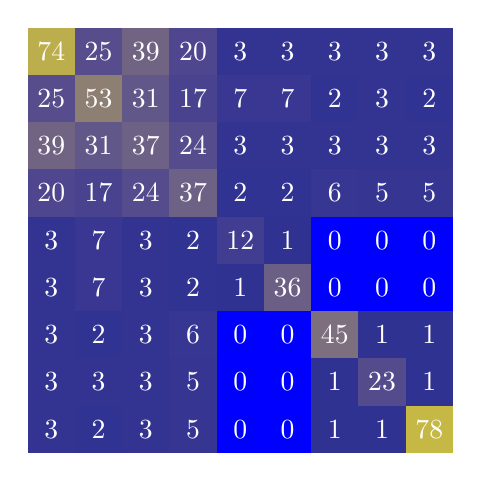
\begin{tikzpicture}[scale=0.6]
  \foreach \y [count=\n] in {
      {74,25,39,20,3,3,3,3,3},
      {25,53,31,17,7,7,2,3,2},
      {39,31,37,24,3,3,3,3,3},
      {20,17,24,37,2,2,6,5,5},
      {3,7,3,2,12,1,0,0,0},
      {3,7,3,2,1,36,0,0,0},
      {3,2,3,6,0,0,45,1,1},
      {3,3,3,5,0,0,1,23,1},
      {3,2,3,5,0,0,1,1,78},
    } {
      \foreach \x [count=\m] in \y {
        \node[fill=yellow!\x!blue, minimum size=6mm, text=white] at (\m,-\n) {\x};
      }
    }
\end{tikzpicture}\quad
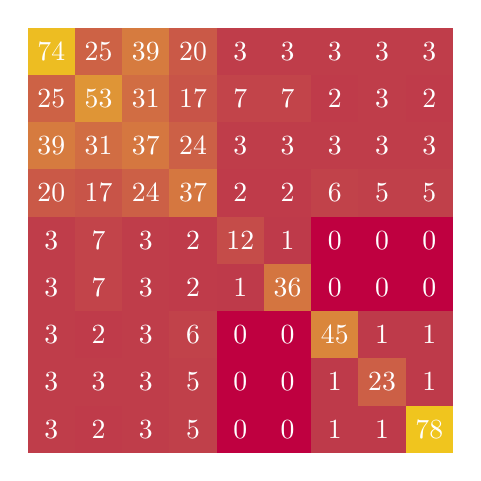
\begin{tikzpicture}[scale=0.6]
  \foreach \y [count=\n] in {
      {74,25,39,20,3,3,3,3,3},
      {25,53,31,17,7,7,2,3,2},
      {39,31,37,24,3,3,3,3,3},
      {20,17,24,37,2,2,6,5,5},
      {3,7,3,2,12,1,0,0,0},
      {3,7,3,2,1,36,0,0,0},
      {3,2,3,6,0,0,45,1,1},
      {3,3,3,5,0,0,1,23,1},
      {3,2,3,5,0,0,1,1,78},
    } {
      \foreach \x [count=\m] in \y {
        \node[fill=yellow!\x!purple, minimum size=6mm, text=white] at (\m,-\n) {\x};
      }
    }
\end{tikzpicture}
}
\caption{图~2的标题名称}
\end{figure}



参考话术:我们需要解决的问题是$\cdots\cdots$,题目要求是$\cdots\cdots$,剔除$\cdots\cdots$数据后选用何种类型的模型优点进行分析。具体步骤123$\cdots$



\subsubsection{***模型的求解}

\textcolor{red}{将预处理数据带入上述模型,通过$\cdots$软件得到$\cdots$结果。(编程代码详见附件*)。模型求解及结果需要图文并茂,用数据说话  用图展示。具体步骤123$\cdots$}
\begin{align}
A_{\max}& =\dfrac{3600}{t_{\min}}=\dfrac{3600}{J_{\min} /(v / 3.6)}
=\dfrac{1000 v}{J_{\min }}(\text{辆 } / h) \\
J_{\min}& =J_{\rm r}+J_{z}+J_{\rm a}
\end{align}


\subsubsection{***结果}

\textcolor{red}{针对于每一个问题的结果综述总结。}



\subsection{问题 三的求解和分析 的求解和分析 的求解和分析}

\subsubsection{对问题的分析}

问题 三要求我们 $\cdots$。

\subsubsection{对问题的求解}

\textbf{模型 Ⅱ—基于 负荷度 负荷度 分析 的小区开放影响度综合评价}

(1)模型的准备

1)负荷度介绍

负荷度( V/CV/CV/C)是指在理想条件下,最大服务交通量与基本行能力之比.

2)数据处理

将道路分为主干和次,其要参数详见 表 10

\begin{table*}[h!]
  \centering
  \small
  \tabcolsep 2.5pt
  \caption{主次道路参数表}
\begin{tabular*}{0.8\linewidth}{p{60pt}<{\centering}p{60pt}<{\centering}
p{60pt}<{\centering}p{80pt}<{\centering}p{80pt}<{\centering}}
\toprule
  道路类型  &  主干路  &  支干路  &  小区内宽道路  &  小区内窄道路  \\
  \midrule
  行车速度  & 50 km / h & 40 km / h & 30 km / h & 20 km / h \\
 车道数  & 4 & 3 & 2 & 1 \\
\bottomrule
  \end{tabular*}
  \label{tab10}
\end{table*}

(2)模型的建立

1)小区的分类

根据小区结构,周边道路分布形状和周边道路车道数的不同,我们将小区分
别分为~4、2、3 类,小区的分类结果详见表~11


2)计算周边各路段及交叉口的通行能力



对于周边各路段的通行能力,我们运用问题二已建立的模型进行计算.在此
基础上对于交叉口的通行能力交叉口~G 我们建立公式如下:

\begin{align}
G_{\text{交又口}}& =\sum_{i=1}^{n} G_{i} \\
G_{i}& =\sum_{j=1}^{k} C_{j}
\end{align}


其中,$C_{j}$ 为进口各车道的通行能力,$ G_{i}$ 为交叉口各进口的通行能力.


3)建立影响度综合评价体系~[9][10][11]

我们采用先单项评价再综合评价的方法,其总体思路见表~12

\begin{table*}[h!]
  \centering
  \small
  \tabcolsep 2.5pt
  \caption{小区分类表}
\begin{tabular*}{0.8\linewidth}{p{100pt}<{\centering}|p{60pt}<{\raggedright}|p{180pt}<{\raggedright}}
\hline
分类标准 & 类型名称& 类型说明\\
\hline
\multirow{4}*{小区结构 }& A组团有序型 & 小区楼房呈组团型分布,每一区域间隔较大,开放后小区
道路较宽,且区域间分布有序\\

& B紧凑有序型 & 小区楼房间隔紧凑,且排列有序,开放后道路网格呈“街
区型”,特点为“高密度、窄路宽.\\
 &C组团无序型& 小区楼房呈组团式分布,每一区域间隔较大,开放后小区
道路较宽,但区域间分布杂乱小区楼房间隔紧凑,但排列杂乱,开放后小区道路呈现“低\\
&D紧凑无序型&密度,窄路宽”的特点\\

\multirow{2}*{周边道路形状分布}& 四周围绕型&四周均为道路\\

&半边包围型&半边围绕道路\\

\multirow{3}*{车道数(针对半封闭性)}& 主干道型 & 两条道路均为主干道\\

&次干道型 & 两条道路均为次干道\\

&混合型& 两条道路一主一次\\
\hline
  \end{tabular*}
  \label{tab11}
\end{table*}

\begin{table*}[h!]
  \centering
  \small
  \tabcolsep 2.5pt
  \caption{综合评价思路表}
\begin{tabular*}{0.8\linewidth}{p{100pt}<{\centering}|p{160pt}<{\raggedright}|p{80pt}<{\raggedright}}
\hline
 评价性质  &  评价内容  &  评价指标  \\
 \hline
\multirow{2}*{ 单项评价 } & \multirow{2}*{  局部路段及交叉口交通负荷影响 } &  路段影响度  \\
& &交叉口影响\\
\multirow{2}*{ 综合评价 } & \multirow{2}*{整个路网交通负荷影响} &平均路段影响度  \\
&&平均交叉口影响度\\
\hline
  \end{tabular*}
  \label{tab12}
\end{table*}

A. 负荷度单项评价

a. 封闭式小区开放后,新增小区内道路对于周边某一路段i 的影响度 $K_{si}$
根据公式计算:
\begin{align}
K_{s i}&=\dfrac{I_{s i p}-I_{s i b}}{B_{s i}} \\
I_{s i p}& =I_{s i b}+a
\end{align}

其中,$I _{sip}$ 为小区道路建成后路段 i 上高峰小时交通量,$I _{sib}$ 为不考虑小区道
 路建成后新增交通量的情况下,路段 i 的高峰小时交通量,  $B_{s i}$  为路段 $i$ 的设计
 通行能力,$a$ 为开放后小区道路的通行量.
b. 封闭式小区开放后,新增小区内道路对于周边道路交叉口的影响度  $K_{c i}$
根据公式计算:
\begin{align}
  K_{c i}=\dfrac{I_{c i p}-I_{c b}}{B_{c t}}
\end{align}


其中,$K_a$ 为小区道路建成后对交叉口 i 的影响度,$I_{crp}$ 为小区道路建成后交 叉口 $i$
上高峰小时交通量, $ I_{c i b}$  为不考虑小区道路建成后新增交通量的情况下, 交叉口 i 的
高峰小时交通量,  $B_{c i}$  为交叉口 $i$ 的设计通行能力.


\begin{figure}[h!t]
\centerline{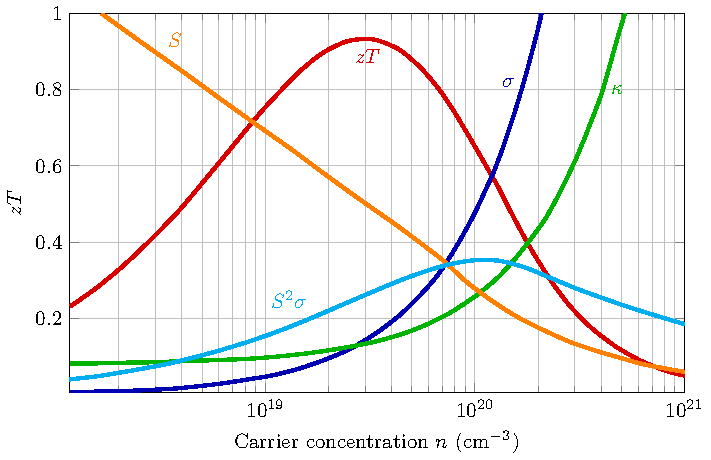
\includegraphics[scale=1]{fig1.pdf}}
\caption{\song\wuhao 图~3的标题名称}
\end{figure}


\section{模型的评价与推广 模型的评价与推广}

\textcolor{red}{将模型进行数值计算,并与附件中的真实采样值(进行列表或图示)比较。对误差进行数据分析,给出误差分析的理论估计。}

\subsection{模型的评价}


1. 优点

\textcolor{red}{得到满意的解、
较好地解决了$\cdots$问题、
使模型得到简化、
使结果更合理,避免…带来的较大误差、
使问题描述比较清晰、
减少大的计算量。
}

(1)问题求解中 辅之流程图, 将建模思路完整清晰的展现出来;

(2)问题二在对 问题二在对理论通行能力进修复时考虑因素 细致、全面,理论通行能力进修复时考虑因素
 细致、全面,系数准确度高;

(3)在问题三中,提出“影响度”的概念较为直观地定量给小区开放后的效果,简便有.在影响度计算上由
点及面从每个路段、交叉口到整 个路网,层深入具有逻辑性;

\begin{figure}[h!t]
\centerline{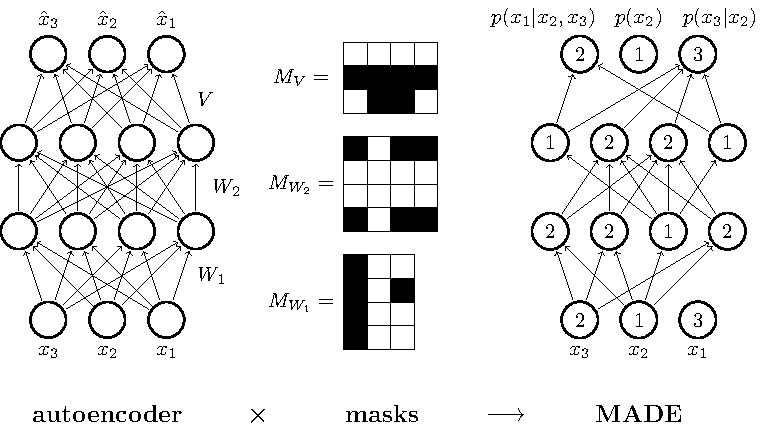
\includegraphics[scale=1]{fig4.pdf}}
\caption{\song\wuhao 图~3的标题名称}
\end{figure}


(4)运用多种数学软件(如 MATLAB、SPSS),取长补短,使计算结果更加),取长补短,使计算结果更
加 准确、明晰.

2. 缺点

\textcolor{red}{主观性过强、
建立在什么的前提条件下、
有一定的局限性、
存在不确定性、
有一定的偏差。
}

(1)在数学软件的计算中会将小数计算 结果进行保留,使得随后的会将小数计算 结果进行保留,使得随后
的或统计结果造成一定误差;

(2)问题二求解修正通行能力时多次使用了查表,操作不够简便.

\subsection{模型的、模型的 推广}

\begin{itemize}

\item \textcolor{red}{对本文中的模型给出比较客观的评价,必须实事求是,有根据,以便评卷人参考。}

\item \textcolor{red}{推广和优化,需要花费功夫想出合理的、甚至可以合理改变题目给出的条件的、不一定可行但是具有一定想象空间的准理想的方法、模型。由此做出一些改进方向,也可以是参赛者一些来不及实现的思路。}
\end{itemize}

1. 问题二中 建立 的模型 在现实 生活 中可以 作为 检验 数据 对实测数据 的准确 性进行 检验,帮助 人们
更好 的测算 交通 数据.

2. 基于问题三建立的模型,可以根据道路实时检测数(某段单位间内 基于问题三建立的模型,推算新建
一条道路对于当前交 通状况的改善效果,帮助度等).

\section{模型的改进}

\subsection{模型一的改进}
针对问题二中的模型一,在具体求解大型车对车辆通行能力的修正系数时,
我们利用交通量的测算值对照得到相应的大型车修正系数.但是,在实际操作中
交通量的测定有很大的难度,如果此时交通量数据无法得到,那么我们便不能得
到相应的修正系数,因此我们对模型进行改进.

由~GREENSHIELD K-V 线性模型,可得通行能力的公式:
\begin{align}
A_{p}=\begin{cases}
\dfrac{3600}{t}\left(1-\dfrac{3.6 l}{V_{t} t}\right)\left(V_{f}>7.2 l / t\right) \\
\dfrac{250 V_{f}}{t}\left(V_{f} \leq 7.2 l / t\right)
\end{cases}
\end{align}

对应的临界车辆速度:
\begin{align}
V_{p}=\begin{cases}
\dfrac{V_{f}-3.6 l}{t} & \left(V_{f}>7.2 l / t\right) \\
\dfrac{1}{2} V_{f} & \left(V_{f} \leq 7.2 l / t\right)
\end{cases}
\end{align}

由美国道路通行能力准则可得,美国将道路服务水平分为六级:A-F 级,而
我国目前针对当前国情,将道路服务水平分成四级:一级相当于美国的A、B 两
级;二级相当于美国的C 级;三级相当于美国的D 级;四级相当于美国的E、F
级。因此,相应的,将美国服务水平划分标准进行针对性修正,得到中国道路服
务水平划分标准,见表

\begin{table*}[h!]
  \centering
  \small
  \tabcolsep 2pt
  \caption{我国服务水平划分标准}
\begin{tabular*}{0.87\linewidth}{p{60pt}<{\centering}p{40pt}<{\centering}
p{40pt}<{\centering}p{40pt}<{\centering}p{40pt}<{\centering}
p{80pt}<{\centering}p{40pt}<{\centering}}
\toprule
服务水平 (L0S)  & \multicolumn{2}{c} {一级 } & 二级  & 三级  & \multicolumn{2}{c} {四级 } \\
\cline{2-3}\cline{6-7}
服务交通量  & 800 & 1200 & 1800 & 2500 & $A_{D}$ & $\leqslant A_{P}$ \\
 速度  km / h & 120 & 120 & 120 & 120 & $\geqslant V_{p}$ & $\leqslant V_{p}$ \\
 V / C & 0.33 & 0.48 & 0.71 & 1.0 & $A_{p} / A_{\max}\leqslant 1.0$ & -(无意义 ) \\
\bottomrule
  \end{tabular*}
\end{table*}

由于车流量的测算相对于交通量来说较易得到,我们便可以不用对交通量进
行测算,可以通过车流量与通行能力的比值计算出~V/C 饱和度值,再通过该值对
照我国服务水平划分标准,间接得到服务交通量,从而得到大型车对通行能力的
修正系数.


\subsection{模型二的改进}

针对于问题三中的模型,在得出各个类型小区在开放后对于整个小区周边路
网交通负荷影响度后,无法判别小区开放的效果是积极的还是消极的,由此我们
可以采用~Bress 悖论的原理进行判别:在个人独立选择路径的情况下,为某路网
增加额外的通行能力(如增加路段的等),反而会导致整个路网的整体运行水平
降低的情况.

将路网进行简化如图~15:

根据推导可得: 当 $\beta_{3}/\left(\beta_{1}+\beta_{2}\right) \leq\left(\beta_{5}+\beta_{6}\right)/\beta_{4}$ 时,会发生悖论,即道路的开
通反而会加剧原有道路的交通状况.

\textcolor{red}{需重新起页,不得与论文正文内容在同一页上}

\begin{rmk}
5篇以上!
\end{rmk}

\newpage

\begin{thebibliography}{99}
\addcontentsline{toc}{section}{参考文献}
\bibitem{1} 李向鹏. 城市交通拥堵对策——封闭型小区交通开放研究~[D]. 交通运输工程,
2014.4.
\bibitem{2} 司守奎等. 数学建模算法与应用~[M]. 北京:国防工业出版社,2011.8 第一版;
\bibitem{3} 吕彬. 城市居住区“开放性”模式研究~[D]. 建筑设计,2006.6.
\bibitem{4} 茹红蕾. 城市道路通行能力的影响因素研究~[D]. 交通运输工程,2008.3.
\bibitem{5} VISSIM 软件路网搭建教程.
\url{http://wenku. baidu.com/view/7bc33214680203d8ce2f24c4.html}
\bibitem{6} 赵琳,邵长桥. 基于~VISSIM 的高速公路基本路段实际通行能力仿真分析~[J]. 道
路交通与安全,2007.2.
\bibitem{7} 李冬梅,李文权. 道路通行能力的计算方法 [J]. 河南大学学报,2002.6:24-27.
\bibitem{8} 城市轨道施工安全及交通组织 [S].2014.
\bibitem{9} 李鑫, 李雪等. 城市道路网络脆弱性评估指标研究综述~[J]. 公路交通科技,
2016.1:155-157.
\bibitem{10} 詹斌, 蔡瑞东等. 基于城市道路网络脆弱性的小区开放策略研究 [J]. 技术方法,
2016.7:98-101.
\bibitem{11} 彭驰. 物流园区交通影响分析研究~[D]. 交通运输工程,2007, 4.

\end{thebibliography}
\newpage

\begin{appendices}

\section*{}

\textbf{\textcolor[rgb]{0.98,0.00,0.00}{程序一:MATLAB算道路车辆通行能力:}}
\lstinputlisting[language=Matlab]{./code/mcmthesis-matlab1.m}

\section*{}

\textcolor[rgb]{0.98,0.00,0.00}{\textbf{程序二:C++ 求解路网正体影响度:}}
\lstinputlisting[language=C++]{./code/mcmthesis-sudoku.cpp}

\newpage
\def\thesection{A}
\renewcommand{\thetable}{\wuhao A-\arabic{table}}
\setcounter{table}{0}
\section*{数据表格}
\textcolor[rgb]{0.98,0.00,0.00}{\textbf{表格数据:}}

\begin{table*}[h!]
  \centering
  \small
    \caption{附表1数据}
\begin{tabular*}{\linewidth}{p{40pt}<{\centering}p{30pt}<{\centering}
p{30pt}<{\centering}p{40pt}<{\centering}p{50pt}<{\centering}p{70pt}<{\centering}
p{60pt}<{\centering}p{50pt}<{\centering}}
\toprule
样本编号 &  车速 & 车道数  & 侧向 净宽 &  车道宽  &  司机反应时间  & 车辆南止耗时  &  交通量  \\
\midrule
1 & 37 {\color{Blue} } & 2 & 1 & 3 & 0.5 & 1.72 & 1112 \\
2 & 47 & 3 & 2.5 & 3.5 & 0.6 & 2.41 & 1835 \\
3 & 48 & 3 & 2.5 & 3.25 & 1.2 & 2.475 & 2034 \\
4 & 44 & 2 & 2.5 & 3.25 & 1 & 2.26 & 1477 \\
5 & 46 & 3 & 2.5 & 3 & 1.2 & 2.27 & 1648 \\
6 & 53 & 2 & 2.5 & 3.5 & 1.2 & 2.498 & 1952 \\
7 & 54 & 3 & 3.5 & 3.5 & 2 & 2.5 & 2249 \\
8 & 59 & 3 & 3.5 & 3.5 & 0.7 & 2.634 & 1893 \\
9 & 59 & 3 & 3.5 & 3.25 & 0.2 & 2.642 & 2245 \\
10 & 48 & 3 & 2.5 & 3.25 & 0.3 & 2.46 & 2035 \\
11 & 50 & 3 & 4.5 & 3.5 & 0.3 & 2.52 & 2318 \\
12 & 56 & 3 & 3.5 & 3.25 & 0.9 & 2.617 & 2203 \\
13 & 57 & 2 & 2.5 & 3.5 & 0.8 & 2.625 & 2034 \\
14 & 58 & 2 & 2.5 & 3 & 0.6 & 2.641 & 2178 \\
15 & 68 & 4 & 3.5 & 3.25 & 0.9 & 3.05 & 2468 \\
16 & 59 & 3 & 4.5 & 3.75 & 0.6 & 2.975 & 2406 \\
17 & 75 & 4 & 4.5 & 3.75 & 0.7 & 3.15 & 2648 \\
18 & 22 & 1 & 1 & 3 & 1.1 & 1.45 & 800 \\
19 & 27 & 4 & 0.5 & 3 & 0.6 & 1.5 & 903 \\
20 & 75 & 1 & 2.5 & 3.5 & 0.6 & 1.46 & 1010 \\
21 & 76 & 1 & 3.5 & 3.5 & 0.2 & 1.63 & 1069 \\
22 & 46 & 2 & 1.5 & 3.25 & 1.9 & 2.3 & 1682 \\
23 & 46 & 2 & 2.5 & 3.25 & 1 & 2.32 & 1734 \\
24 & 46 & 2 & 2.5 & 3.75 & 0.2 & 2.4 & 1826 \\
25 & 47 & 3 & 2.5 & 3.25 & 1.2 & 2.37 & 1625 \\
26 & 77 & 3 & 4.5 & 3.5 & 0.2 & 2.475 & 2148 \\
27 & 48 & 3 & 4.5 & 3.25 & 0.3 & 2.47 & 2278 \\
28 & 80 & 3 & 2.5 & 3.5 & 0.5 & 2.58 & 2177 \\
29 & 66 & 2 & 3.5 & 3.5 & 1 & 2.72 & 2249 \\
30 & 67 & 4 & 3.5 & 3.75 & 0.9 & 2.975 & 2484 \\
31 & 25 & 3 & 1.5 & 3.5 & 0.6 & 1.3 & 846 \\
32 & 34 & 2 & 4.5 & 3.5 & 0.8 & 1.52 & 1152 \\
33 & 47 & 3 & 2.5 & 3.25 & 0.3 & 2.42 & 1753 \\
34 & 48 & 4 & 2.5 & 3.75 & 0.3 & 2.34 & 1924 \\
35 & 79 & 3 & 2.5 & 3.25 & 1.1 & 2.53 & 2159 \\
36 & 55 & 3 & 0.5 & 3.5 & 0.9 & 2.62 & 1568 \\
37 & 78 & 2 & 1 & 3.5 & 0.9 & 2.618 & 2148 \\
38 & 59 & 3 & 1 & 3.5 & 1 & 2.64 & 2272 \\
39 & 19 & 1 & 0 & 3 & 1.2 & 1.4 & 513 \\
40 & 19 & 2 & 2.5 & 3.25 & 1 & 1.35 & 810 \\
41 & 37 & 2 & 2.5 & 3 & 1.2 & 1.49 & 1102 \\
42 & 45 & 2 & 2.5 & 3.5 & 0.8 & 2.28 & 1525 \\
\bottomrule
  \end{tabular*}
  \label{Ap1}
\end{table*}

\newpage

\begin{table*}[h!]
  \centering
  \small
  \caption{小区开放前VISSIM正常行驶仿真数据记录表1}
\begin{tabular*}{\linewidth}{p{40pt}<{\centering}p{30pt}<{\centering}
p{30pt}<{\centering}p{40pt}<{\centering}p{50pt}<{\centering}p{70pt}<{\centering}
p{60pt}<{\centering}p{50pt}<{\centering}}
\toprule
样本编号 &  车速 & 车道数  & 侧向 净宽 &  车道宽  &  司机反应时间  & 车辆南止耗时  &  交通量  \\
\midrule
47 & 67 & 1 & 0.5 & 3.75 & 0.2 & 2.83 & 2249 \\
48 & 67 & 4 & 3.5 & 3.25 & 0.6 & 2.815 & 2463 \\
49 & 75 & 2 & 3.5 & 3.5 & 0.6 & 3.21 & 2748 \\
50 & 34 & 2 & 1.5 & 3 & 1 & 1.48 & 957 \\
51 & 39 & 2 & 2.5 & 3.5 & 0.8 & 1.97 & 1364 \\
52 & 40 & 3 & 2.5 & 3.25 & 0.5 & 2 & 1359 \\
53 & 50 & 3 & 2.5 & 3.5 & 1 & 2.51 & 2264 \\
54 & 55 & 2 & 3.5 & 3.25 & 1.2 & 2.6 & 1978 \\
55 & 55 & 3 & 3.5 & 3.5 & 0.6 & 2.61 & 2218 \\
56 & 59 & 3 & 0.5 & 3 & 0.2 & 2.638 & 1974 \\
57 & 63 & 4 & 2.5 & 3.5 & 1.1 & 2.78 & 2384 \\
58 & 67 & 3 & 2.5 & 3.75 & 0.8 & 2.83 & 2384 \\
59 & 75 & 3 & 4.5 & 3.5 & 0.3 & 3.2 & 2801 \\
60 & 77 & 2 & 4.5 & 3.5 & 0.2 & 3.18 & 2845 \\
61 & 23 & 1 & 0 & 3 & 0.5 & 1.44 & 458 \\
62 & 75 & 2 & 1 & 3 & 0.2 & 1.625 & 1065 \\
63 & 46 & 2 & 2.5 & 3.5 & 1 & 2.43 & 1752 \\
64 & 61 & 2 & 0.5 & 3 & 1.2 & 2.71 & 1890 \\
65 & 36 & 3 & 2.5 & 3.5 & 1 & 1.67 & 1233 \\
66 & 38 & 2 & 3.5 & 3 & 1.7 & 1.9 & 1246 \\
67 & 55 & 1 & 0.5 & 3.5 & 0.3 & 2.615 & 1763 \\
68 & 74 & 2 & 1.5 & 3.75 & 0.7 & 3.05 & 2349 \\
69 & 79 & 4 & 2.5 & 3.75 & 0.4 & 3.17 & 2694 \\
70 & 38 & 2 & 3.5 & 3 & 1.1 & 1.86 & 1343 \\
71 & 61 & 3 & 1.5 & 3.25 & 0.3 & 2.68 & 2006 \\
72 & 79 & 3 & 3.5 & 3.5 & 2.1 & 3.48 & 2948 \\
73 & 27 & 2 & 1 & 3.75 & 0.8 & 1.48 & 928 \\
74 & 28 & 1 & 1 & 3 & 0.9 & 1.47 & 947 \\
75 & 34 & 2 & 1 & 3 & 0.3 & 1.49 & 998 \\
76 & 44 & 3 & 2.5 & 3.25 & 0.3 & 2.24 & 1520 \\
77 & 78 & 3 & 4.5 & 3.5 & 0.7 & 3.09 & 2648 \\
78 & 73 & 3 & 3.5 & 3.5 & 1.2 & 3.19 & 2741 \\
80 & 37 & 4 & 1 & 3 & 1.7 & 1.87 & 1265 \\
81 & 37 & 2 & 3.5 & 3.5 & 1.5 & 1.84 & 1325 \\
82 & 38 & 2 & 2.5 & 3 & 1.2 & 1.95 & 1233 \\
83 & 38 & 2 & 1 & 3 & 2.1 & 1.97 & 1249 \\
84 & 40 & 2 & 1.5 & 3 & 0.4 & 2.12 & 1366 \\
85 & 42 & 3 & 4.5 & 3.75 & 0.4 & 2.16 & 1638 \\
86 & 40 & 3 & 1.5 & 3.25 & 0.8 & 2.43 & 1384 \\
87 & 41 & 3 & 1.5 & 3.5 & 1.1 & 2.05 & 1434 \\
88 & 78 & 3 & 4.5 & 3.75 & 1.4 & 3.42 & 3048 \\
89 & 41 & 4 & 1.5 & 3.75 & 0.8 & 2.15 & 1566 \\
90 & 42 & 2 & 4.5 & 3.25 & 1.8 & 2.2 & 1466 \\
91 & 44 & 2 & 2.5 & 3 & 1.2 & 2.24 & 1475 \\
92 & 75 & 4 & 4.5 & 3.75 & 1.8 & 3.25 & 2801 \\
93 & 37 & 4 & 4.5 & 3.75 & 0.2 & 1.5 & 2043 \\
94 & 37 & 2 & 1 & 3 & 2.1 & 1.89 & 1289 \\
95 & 40 & 4 & 2.5 & 3.5 & 0.9 & 2.15 & 1406 \\
\bottomrule
  \end{tabular*}
  \label{Ap2}
\end{table*}



\begin{table*}[h!]
  \centering
  \small
  \caption{小区开放前VISSIM正常行驶仿真数据记录表2}
\begin{tabular*}{\linewidth}{p{40pt}<{\centering}p{30pt}<{\centering}
p{30pt}<{\centering}p{40pt}<{\centering}p{50pt}<{\centering}p{70pt}<{\centering}
p{60pt}<{\centering}p{50pt}<{\centering}}
\toprule
样本编号 &  车速 & 车道数  & 侧向 净宽 &  车道宽  &  司机反应时间  & 车辆南止耗时  &  交通量  \\
\midrule
47 & 67 & 1 & 0.5 & 3.75 & 0.2 & 2.83 & 2249 \\
48 & 67 & 4 & 3.5 & 3.25 & 0.6 & 2.815 & 2463 \\
49 & 75 & 2 & 3.5 & 3.5 & 0.6 & 3.21 & 2748 \\
50 & 34 & 2 & 1.5 & 3 & 1 & 1.48 & 957 \\
51 & 39 & 2 & 2.5 & 3.5 & 0.8 & 1.97 & 1364 \\
52 & 40 & 3 & 2.5 & 3.25 & 0.5 & 2 & 1359 \\
53 & 50 & 3 & 2.5 & 3.5 & 1 & 2.51 & 2264 \\
54 & 55 & 2 & 3.5 & 3.25 & 1.2 & 2.6 & 1978 \\
55 & 55 & 3 & 3.5 & 3.5 & 0.6 & 2.61 & 2218 \\
56 & 59 & 3 & 0.5 & 3 & 0.2 & 2.638 & 1974 \\
57 & 63 & 4 & 2.5 & 3.5 & 1.1 & 2.78 & 2384 \\
58 & 67 & 3 & 2.5 & 3.75 & 0.8 & 2.83 & 2384 \\
59 & 75 & 3 & 4.5 & 3.5 & 0.3 & 3.2 & 2801 \\
60 & 77 & 2 & 4.5 & 3.5 & 0.2 & 3.18 & 2845 \\
61 & 23 & 1 & 0 & 3 & 0.5 & 1.44 & 458 \\
62 & 75 & 2 & 1 & 3 & 0.2 & 1.625 & 1065 \\
63 & 46 & 2 & 2.5 & 3.5 & 1 & 2.43 & 1752 \\
64 & 61 & 2 & 0.5 & 3 & 1.2 & 2.71 & 1890 \\
65 & 36 & 3 & 2.5 & 3.5 & 1 & 1.67 & 1233 \\
66 & 38 & 2 & 3.5 & 3 & 1.7 & 1.9 & 1246 \\
67 & 55 & 1 & 0.5 & 3.5 & 0.3 & 2.615 & 1763 \\
68 & 74 & 2 & 1.5 & 3.75 & 0.7 & 3.05 & 2349 \\
69 & 79 & 4 & 2.5 & 3.75 & 0.4 & 3.17 & 2694 \\
70 & 38 & 2 & 3.5 & 3 & 1.1 & 1.86 & 1343 \\
71 & 61 & 3 & 1.5 & 3.25 & 0.3 & 2.68 & 2006 \\
72 & 79 & 3 & 3.5 & 3.5 & 2.1 & 3.48 & 2948 \\
73 & 27 & 2 & 1 & 3.75 & 0.8 & 1.48 & 928 \\
74 & 28 & 1 & 1 & 3 & 0.9 & 1.47 & 947 \\
75 & 34 & 2 & 1 & 3 & 0.3 & 1.49 & 998 \\
76 & 44 & 3 & 2.5 & 3.25 & 0.3 & 2.24 & 1520 \\
77 & 78 & 3 & 4.5 & 3.5 & 0.7 & 3.09 & 2648 \\
78 & 73 & 3 & 3.5 & 3.5 & 1.2 & 3.19 & 2741 \\
80 & 37 & 4 & 1 & 3 & 1.7 & 1.87 & 1265 \\
81 & 37 & 2 & 3.5 & 3.5 & 1.5 & 1.84 & 1325 \\
82 & 38 & 2 & 2.5 & 3 & 1.2 & 1.95 & 1233 \\
83 & 38 & 2 & 1 & 3 & 2.1 & 1.97 & 1249 \\
84 & 40 & 2 & 1.5 & 3 & 0.4 & 2.12 & 1366 \\
85 & 42 & 3 & 4.5 & 3.75 & 0.4 & 2.16 & 1638 \\
86 & 40 & 3 & 1.5 & 3.25 & 0.8 & 2.43 & 1384 \\
87 & 41 & 3 & 1.5 & 3.5 & 1.1 & 2.05 & 1434 \\
88 & 78 & 3 & 4.5 & 3.75 & 1.4 & 3.42 & 3048 \\
89 & 41 & 4 & 1.5 & 3.75 & 0.8 & 2.15 & 1566 \\
90 & 42 & 2 & 4.5 & 3.25 & 1.8 & 2.2 & 1466 \\
91 & 44 & 2 & 2.5 & 3 & 1.2 & 2.24 & 1475 \\
92 & 75 & 4 & 4.5 & 3.75 & 1.8 & 3.25 & 2801 \\
93 & 37 & 4 & 4.5 & 3.75 & 0.2 & 1.5 & 2043 \\
94 & 37 & 2 & 1 & 3 & 2.1 & 1.89 & 1289 \\
95 & 40 & 4 & 2.5 & 3.5 & 0.9 & 2.15 & 1406 \\
\bottomrule
  \end{tabular*}
  \label{Ap3}
\end{table*}

\begin{table*}[h!]
  \centering
  \small
  \caption{小区开放前VISSIM正常行驶仿真数据记录表3}
\begin{tabular*}{\linewidth}{p{50pt}<{\centering}p{50pt}<{\centering}
p{60pt}<{\centering}p{60pt}<{\centering}p{60pt}<{\centering}p{70pt}<{\centering}}
\toprule
 数据P.C. & 时间(进入) & 时间(离开) & 车辆编号& 速度(m/s) & 车辆长度(m) \\
\midrule
1 & 9.34 & -1 & 4 & 14.7 & 4.76 \\
1 & -1 & 9.67 & 4 & 14.7 & 4.76 \\
7 & 19.34 & -1 & 3 & 14.7 & 4.76 \\
7 & -1 & 19.66 & 3 & 14.8 & 4.76 \\
6 & 20.35 & -1 & 4 & 14 & 4.76 \\
6 & -1 & 20.69 & 4 & 14 & 4.76 \\
1 & 21.49 & -1 & 11 & 14.8 & 4.61 \\
2 & 21.43 & -1 & 5 & 15.9 & 4.55 \\
1 & -1 & 21.8 & 11 & 14.9 & 4.61 \\
2 & -1 & 21.72 & 5 & 15.9 & 4.55 \\
5 & 22.36 & -1 & 6 & 15.4 & 4.61 \\
5 & -1 & 22.66 & 6 & 15.4 & 4.61 \\
2 & 25.81 & -1 & 7 & 13.8 & 4.11 \\
2 & -1 & 26.11 & 7 & 13.8 & 4.11 \\
2 & 27.19 & -1 & 8 & 14.1 & 10.21 \\
2 & -1 & 27.92 & 8 & 14.2 & 10.21 \\
7 & 29.24 & -1 & 10 & 15.1 & 4.76 \\
7 & -1 & 29.55 & 10 & 15.1 & 4.76 \\
6 & 32.23 & -1 & 11 & 14.5 & 4.61 \\
6 & -1 & 32.55 & 11 & 14.6 & 4.61 \\
5 & 35.38 & -1 & 12 & 14.8 & 4.55 \\
5 & -1 & 35.68 & 12 & 14.9 & 4.55 \\
7 & 36.42 & -1 & 13 & 14.5 & 4.55 \\
7 & -1 & 36.73 & 13 & 14.5 & 4.55 \\
1 & 38.87 & -1 & 16 & 15.4 & 4.61 \\
1 & -1 & 39.16 & 16 & 15.4 & 4.61 \\
6 & 49.09 & -1 & 16 & 15.1 & 4.61 \\
6 & -1 & 49.4 & 16 & 15.1 & 4.61 \\
1 & 49.91 & -1 & 24 & 15.1 & 4.55 \\
1 & -1 & 50.21 & 24 & 15.2 & 4.55 \\
5 & 50.59 & -1 & 17 & 15.3 & 4.55 \\
5 & -1 & 50.89 & 17 & 15.3 & 4.55 \\
3 & 56.27 & -1 & 14 & 15.8 & 4.76 \\
3 & -1 & 56.57 & 14 & 15.9 & 4.76 \\
7 & 57.12 & -1 & 23 & 15.9 & 4.76 \\
7 & -1 & 57.42 & 23 & 15.8 & 4.76 \\
6 & 60.56 & -1 & 24 & 14.6 & 4.55 \\
6 & -1 & 60.87 & 24 & 14.7 & 4.55 \\
3 & 63.02 & -1 & 18 & 15.1 & 4.11 \\
3 & -1 & 63.29 & 18 & 15.1 & 4.11 \\
3 & 66.53 & -1 & 15 & 15 & 4.11 \\
1 & 66.65 & -1 & 33 & 15 & 4.4 \\
1 & -1 & 66.94 & 33 & 15.1 & 4.4 \\
3 & -1 & 66.8 & 15 & 14.9 & 4.11 \\
5 & 67.35 & -1 & 28 & 14.7 & 4.76 \\
5 & -1 & 67.68 & 28 & 14.7 & 4.76 \\
\bottomrule
  \end{tabular*}
  \label{Ap3}
\end{table*}

\newpage

\begin{table*}[h!]
  \centering
  \small
  \caption{小区开放前VISSIM正常行驶仿真数据记录表1}
\begin{tabular*}{\linewidth}{p{50pt}<{\centering}p{50pt}<{\centering}
p{60pt}<{\centering}p{60pt}<{\centering}p{60pt}<{\centering}p{70pt}<{\centering}}
\toprule
 数据P.C. & 时间(进入) & 时间(离开) & 车辆编号& 速度(m/s) & 车辆长度(m) \\
\midrule
5 & -1 & 80.44 & 35 & 15 & 4.55 \\
7 & 84.64 & -1 & 37 & 14.5 & 10.21 \\
7 & -1 & 85.35 & 37 & 14.4 & 10.21 \\
3 & 89.77 & -1 & 31 & 14.7 & 4.76 \\
3 & -1 & 90.09 & 31 & 14.8 & 4.76 \\
2 & 90.42 & -1 & 32 & 15.2 & 4.11 \\
2 & -1 & 90.69 & 32 & 15.2 & 4.11 \\
1 & 90.84 & -1 & 40 & 1.7 & 11.54 \\
3 & 93.85 & -1 & 34 & 13.9 & 4.76 \\
3 & -1 & 94.19 & 34 & 14 & 4.76 \\
1 & -1 & 98.34 & 40 & 1.8 & 11.54 \\
1 & 101.18 & -1 & 44 & 3.5 & 4.4 \\
2 & 101.41 & -1 & 29 & 14.6 & 4.61 \\
2 & -1 & 101.73 & 29 & 14.5 & 4.61 \\
1 & -1 & 101.8 & 44 & 4.3 & 4.4 \\
3 & 103.39 & -1 & 36 & 14.5 & 4.76 \\
3 & -1 & 103.72 & 36 & 1.5 & 4.76 \\
2 & 109.33 & -1 & 39 & 15.7 & 4.76 \\
2 & -1 & 109.63 & 39 & 15.7 & 4.76 \\
1 & 113.78 & -1 & 52 & 3.3 & 4.11 \\
1 & -1 & 114.75 & 52 & 5.6 & 4.11 \\
6 & 116.66 & -1 & 46 & 15 & 4.4 \\
6 & -1 & 116.96 & 46 & 15 & 4.4 \\
4 & 117.67 & -1 & 1 & 2 & 0.44 \\
4 & -1 & 117.89 & 1 & 2 & 0.44 \\
6 & 119.37 & -1 & 44 & 14.2 & 4.4 \\
6 & -1 & 119.68 & 44 & 14.1 & 4.4 \\
1 & 127.94 & -1 & 56 & 1.2 & 0.34 \\
1 & -1 & 128.22 & 56 & 1.2 & 0.34 \\
3 & 128.54 & -1 & 45 & 12.7 & 4.34 \\
3 & -1 & 128.87 & 45 & 13 & 4.34 \\
4 & 128.86 & -1 & 38 & 3.4 & 1.45 \\
4 & -1 & 129.28 & 38 & 3.5 & 1.45 \\
6 & 132.61 & -1 & 52 & 14.2 & 4.11 \\
1 & 132.94 & -1 & 60 & 1.6 & 4.4 \\
1 & 101.18 & -1 & 44 & 3.5 & 4.4 \\
2 & 101.41 & -1 & 29 & 14.6 & 4.61 \\
2 & -1 & 101.73 & 29 & 14.5 & 4.61 \\
1 & -1 & 101.8 & 44 & 4.3 & 4.4 \\
3 & 103.39 & -1 & 36 & 14.5 & 4.76 \\
3 & -1 & 103.72 & 36 & 1.5 & 4.76 \\
2 & 109.33 & -1 & 39 & 15.7 & 4.76 \\
2 & -1 & 109.63 & 39 & 15.7 & 4.76 \\
1 & 113.78 & -1 & 52 & 3.3 & 4.11 \\
1 & -1 & 114.75 & 52 & 5.6 & 4.11 \\
6 & 116.66 & -1 & 46 & 15 & 4.4 \\
\bottomrule
  \end{tabular*}
  \label{Ap4}
\end{table*}



\begin{table*}[h!]
  \centering
  \small
  \caption{小区开放前VISSIM正常行驶仿真数据记录表2}
\begin{tabular*}{\linewidth}{p{50pt}<{\centering}p{50pt}<{\centering}
p{60pt}<{\centering}p{60pt}<{\centering}p{60pt}<{\centering}p{70pt}<{\centering}}
\toprule
 数据P.C. & 时间(进入) & 时间(离开) & 车辆编号& 速度(m/s) & 车辆长度(m) \\
\midrule
1 & 127.94 & -1 & 56 & 1.2 & 0.34 \\
1 & -1 & 128.22 & 56 & 1.2 & 0.34 \\
3 & 128.54 & -1 & 45 & 12.7 & 4.34 \\
3 & -1 & 128.87 & 45 & 13 & 4.34 \\
4 & 128.86 & -1 & 38 & 3.4 & 1.45 \\
4 & -1 & 129.28 & 38 & 3.5 & 1.45 \\
2 & -1 & 90.69 & 32 & 15.2 & 4.11 \\
1 & 90.84 & -1 & 40 & 1.7 & 11.54 \\
3 & 93.85 & -1 & 34 & 13.9 & 4.76 \\
3 & -1 & 94.19 & 34 & 14 & 4.76 \\
1 & -1 & 98.34 & 40 & 1.8 & 11.54 \\
1 & 101.18 & -1 & 44 & 3.5 & 4.4 \\
2 & 101.41 & -1 & 29 & 14.6 & 4.61 \\
2 & -1 & 101.73 & 29 & 14.5 & 4.61 \\
1 & -1 & 101.8 & 44 & 4.3 & 4.4 \\
3 & 103.39 & -1 & 36 & 14.5 & 4.76 \\
3 & -1 & 103.72 & 36 & 1.5 & 4.76 \\
2 & 109.33 & -1 & 39 & 15.7 & 4.76 \\
2 & -1 & 109.63 & 39 & 15.7 & 4.76 \\
1 & 113.78 & -1 & 52 & 3.3 & 4.11 \\
1 & -1 & 114.75 & 52 & 5.6 & 4.11 \\
6 & 116.66 & -1 & 46 & 15 & 4.4 \\
6 & -1 & 116.96 & 46 & 15 & 4.4 \\
4 & 117.67 & -1 & 1 & 2 & 0.44 \\
4 & -1 & 117.89 & 1 & 2 & 0.44 \\
6 & 119.37 & -1 & 44 & 14.2 & 4.4 \\
6 & -1 & 119.68 & 44 & 14.1 & 4.4 \\
1 & 127.94 & -1 & 56 & 1.2 & 0.34 \\
1 & -1 & 128.22 & 56 & 1.2 & 0.34 \\
3 & 128.54 & -1 & 45 & 12.7 & 4.34 \\
3 & -1 & 128.87 & 45 & 13 & 4.34 \\
4 & 128.86 & -1 & 38 & 3.4 & 1.45 \\
4 & -1 & 129.28 & 38 & 3.5 & 1.45 \\
6 & 132.61 & -1 & 52 & 14.2 & 4.11 \\
1 & 132.94 & -1 & 60 & 1.6 & 4.4 \\
1 & 101.18 & -1 & 44 & 3.5 & 4.4 \\
2 & 101.41 & -1 & 29 & 14.6 & 4.61 \\
2 & -1 & 101.73 & 29 & 14.5 & 4.61 \\
1 & -1 & 101.8 & 44 & 4.3 & 4.4 \\
3 & 103.39 & -1 & 36 & 14.5 & 4.76 \\
3 & -1 & 103.72 & 36 & 1.5 & 4.76 \\
2 & -1 & 109.63 & 39 & 15.7 & 4.76 \\
1 & 113.78 & -1 & 52 & 3.3 & 4.11 \\
1 & -1 & 114.75 & 52 & 5.6 & 4.11 \\
6 & 116.66 & -1 & 46 & 15 & 4.4 \\
6 & -1 & 116.96 & 46 & 15 & 4.4 \\
\bottomrule
  \end{tabular*}
  \label{Ap4}
\end{table*}







\end{appendices}
\end{document}
%%
%% This work consists of these files mcmthesis.dtx,
%%                                   figures/ and
%%                                   code/,
%% and the derived files             mcmthesis.cls,
%%                                   mcmthesis-demo.tex,
%%                                   README,
%%                                   LICENSE,
%%                                   mcmthesis.pdf and
%%                                   mcmthesis-demo.pdf.
%%
%% End of file `mcmthesis-demo.tex'.
